%
% General structure for the revdetua class:
%
\documentclass[longpaper, english, final, times]{revdetua}
%
% Valid options are:
%
%   longpaper --------- \part and \tableofcontents defined
%   shortpaper -------- \part and \tableofcontents not defined (default)
%
%   english ----------- main language is English (default)
%   portugues --------- main language is Portuguese
%
%   draft ------------- draft version
%   final ------------- final version (default)
%
%   times ------------- use times (postscript) fonts for text
%
%   mirror ------------ prints a mirror image of the paper (with dvips)
%
%   visiblelabels ----- \SL, \SN, \SP, \EL, \EN, etc. defined
%   invisiblelabels --- \SL, \SN, \SP, \EL, \EN, etc. not defined (default)
%
% Note: the final version should use the times fonts
% Note: the really final version should also use the mirror option
%

\usepackage{amsmath}
\usepackage{enumitem}
\usepackage{booktabs} % To thicken table lines
%\usepackage{longtable}
\usepackage{arydshln}
\usepackage{graphicx}


%% ALGORITHM 1 PROCEEDURES-----------------------------------------
%\usepackage{algorithm}
%%\usepackage[algo2e]{algorithm2e} 
%\usepackage{arevmath}     % For math symbols
%\usepackage[noend]{algpseudocode}

%% ALGORITHM 2 FUNCTIONS-----------------------------------------
\usepackage{xcolor}
\usepackage[linesnumbered,ruled,vlined]{algorithm2e}
% set comment color to blue
\newcommand\mycommfont[1]{\footnotesize\ttfamily\textcolor{blue}{#1}}
\SetCommentSty{mycommfont}
\begin{document}
	
	%\Header{Volume}{Number}{Month}{Year}{InitialPage}
	% Note: the month must be in Portuguese
	
	\title{The Minimum Cut Problem For An Undirected Graph}
	\author{ABLORDEPPEY Prosper} % or \author{... \and ...}
	\maketitle
	
	\begin{abstract}% Note: in English
		In this context, given an undirected graph $\mathcal{G(V, E)}$, with $n=\mathcal{|V|}$ vertices and $m=\mathcal{|E|}$ edges, a minimum cut of $\mathcal{G}$ is a partition of the graph's vertices into two complementary sets $S$ and $T$, such that the number of edges between the set $S$ and the set $T$ is as small as possible.
		This presentation studies this problem by designing and testing an exhaustive search algorithm to solve it, as well as an algorithm using a greedy heuristics. A probabilistic randomized technique was also proposed, analyzed and improved so as to obtain the exact minimum cut of interest.
	\end{abstract}
	
%	\begin{resumo}% Note: in Portuguese
%		...
%	\end{resumo}
	
%	\begin{keywords}% Note: in English (optional)
%		...
%	\end{keywords}
	
%	\begin{palavraschave}% Note: in Portuguese (optional)
%		...
%	\end{palavraschave}

	\section{Notation and Problem Definition}
		Consider an undirected graph $\mathcal{G(V,E,W)}$ with $n=|\mathcal{\mathcal{V}}|$ vertices and $m=|\mathcal{E}|$ edges where $w(\{u,v\}) \in \mathcal{W}$ is the number of edges connecting vertex $u$ and vertex $v$ for $(u,v)\in \mathcal{E}$. 
		\begin{itemize}
			\item Let $Adj(\mathcal{G})$ be the adjacency matrix of graph $\mathcal{G}$. $Adj(\mathcal{G})$ is a two dimensional (2D) matrix of ones and zeros where a one (1) indicates the presence of the corresponding edge in the network \cite{adjacencymatrixdefinition}. Suppose $a_{ij}$ is an entry of the $Adj(\mathcal{G})$. Then
			\[
				a_{ij} = 
				\begin{cases} 
					1 & \text{if there is an edge from vertex } j \text{ to vertex } i \\
					0 & \text{otherwise} 
				\end{cases}
			\] 
			\item Let  $vset=\{S, T\}	$ be a complementary partition of $\mathcal{V}$ then
					\[
						S\cup T = \mathcal{V} , S\cap T=\emptyset
					\]
			\item We can define the set of cut edges as
				\[
					C=\left\{(u,v) \in \mathcal{E} | u \in S, v \in T \right\}
				\]
			\item The cut size 
				\[
					\Theta(vset) = \sum_{\{u,v\}\in C}^{} w(\{u,v\})
				\]
				which is equal to the cardinality of $C$ if all edges have unitary weights but different otherwise.
			\item A group of vertices collapsed into one (1) is termed as a \textit{supernode}.
			\item An edge connecting from a supernode to another vertex is called, a \textit{superedge}.
			\item The weight of a superedge is the sum of weights of all individual vertices connecting both supernodes. 
			\item All graphs $\mathcal{G}$ considered in this presentation are connected. Thus, there exists at least one (1) edge between any two (2) vertices of $\mathcal{V}$. 
%			\item Degree of a vertex $u$ represented as $Deg(u)$ is the number of edges connecting vertex $u$ to its immediate neighbors.
		\end{itemize}
	
	\section{Outline Of Implementation}
		The outline of this project is given as follows
		\begin{enumerate}[label=(\arabic*)]
			\item[(III)] describes the Brute-Force or Exhaustive-Search implementation.
			\item[(IV)] describes the implementation of a Greedy-Heuristic technique.
			\item[(V)] implements a random probabilistic approach to estimate the minimum cut. An improved implementation which offers a higher chance of realizing the exact minimum cut compared to the naive method was also proposed.
			\item[(VI)] complexities analysis.
			\item[(VII)] auxiliary functions 
		\end{enumerate}
	 	
	 \section{Brute-Force / Exhaustive Implementation}
		This technique computes the $cut$ for all possible complementary partitions of the vertices set $\mathcal{V}$. The minimum of all these computed cuts represents the $minimum \text{ } cut$ of the graph $\mathcal{G}$. The implementation is presented in Algorithm (\ref{algorithm:ExhaustiveSearchMain}) below with two helping methods \textbf{GetPartCut} as Algorithm (\ref{algorithm:GetPartCut}) and \textbf{GetCompPartitions} as Algorithm (\ref{algorithm:GetCompPartitions}) described below in detail.
		
%		\begin{enumerate}[label=(\arabic*)]
%			\item \textbf{GetPartCut}
			\subsection{Compute Partition Cut}
				\begin{algorithm}
					\caption{Compute Cut Of A Partition of $\mathcal{V}$}
					\label{algorithm:GetPartCut}
					
					% Defining output and inputs
					\SetKwInOut{Input}{Input}  
					\Input{$Adj(\mathcal{G})$ \tcp*{adjacency matrix of $\mathcal{G}$}\\%%
						$S$ \tcp*{$1^{st}$ partition element of $vset$}\\
						$T$ \tcp*{$2^{nd}$ partition element of $vset$}\\  
					}
					\SetKwInput{KwOutput}{Output}              % set the Output
					\DontPrintSemicolon
					
					\KwOutput{Cut} 
					
					% Set Function Names
					\SetKwFunction{FMain}{GetPartCut}
					
					% Function Definition			
					\SetKwProg{Fn}{Function}{:}{\KwRet}
					\Fn{\FMain}{
						$Num\_Cuts \gets$ 0 \;
						\ForEach{$v_1 \in \mathbf{S}$}{%
							\ForEach{$v_2 \in \mathbf{T}$}{%
								\tcp{check if $(v_1,v_2)\in \mathcal{E}$}					
								\uIf{$edge([v_1,v_2]) \in Adj(\mathcal{G})$}{
									$Num\_Cuts = Num\_Cuts + 1$ \;
								}
							}
						}
						\KwRet $Num\_Cuts$\;
					}
				\end{algorithm}
				
				This function returns the cut for a given complementary partition. There are a few other ways to generate the cut of a complementary partition. The logic behind most of them is to contract/merge all vertices of each partition set into supernodes. The weight/cut of the superedge connecting both supernodes then represents the sum of the weights of all contributing edges to some node.\\
				
				The one proposed in this project made use of the adjacency matrix $(Adj(\mathcal{G}))$, which happens to be very straight forward and has easy implementation. The cut for a partition $vset$ is the number of edges connecting $S$ and $T$. To achieve this, we leverage the fact that if an edge exists between two vertices $(v_1, v_2)$, then, their representation/value in the adjacency matrix is one (1). If this is achieved, the number of cuts ($Num\_Cuts$) is updated by one (1).\\
				
				The cut for the given complementary partition will be returned after the end of execution of Algorithm (\ref{algorithm:GetPartCut}). This algorithm runs in $\mathcal{O}(|S|\cdot |T|)$ time. The complexity for this algorithm is analyzed below for the two possible cases where the number of vertices $n$ is even or odd. 
				\begin{itemize}
					\label{list:getpartcut}
					\item If $|\mathcal{V}|=n$ is even
					\begin{align*}
						C = & \mathcal{O}\left(|S|\cdot|T|\right)\\
						= & \mathcal{O}\left(\frac{n}{2}\cdot \frac{n}{2}\right)\\
						= & \mathcal{O}\left(\dfrac{n^2}{4}\right) = \mathcal{O}(n^2)
					\end{align*}
					\item If $|\mathcal{V}|=n$ is odd
					\begin{align*}
						C = & \mathcal{O}\left(|S|\cdot |T|\right)\\
						= & \mathcal{O}\left(\frac{n-1}{2}\cdot \frac{n+1}{2}\right)\\
						= & \mathcal{O}\left(\dfrac{n(n-1)}{4}\right) \\
						= & \mathcal{O}\left(\dfrac{n^2-n}{4}\right)  = \mathcal{O}(n^2)
					\end{align*}
				\end{itemize}
				Hence, for all cases of $n$ the complexity of this algorithm is $\mathbf{\mathcal{O}(n^2)}$.\\
			
%			\item \textbf{GetCompPartitions}
		\subsection{Generate Valid Complementary Partitions}
			\begin{algorithm}[h]
				\caption{Get Valid Compl. Partitions Of $\mathcal{V}$}
				\label{algorithm:GetCompPartitions}
				\SetKwInput{KwInput}{Input}                % Set the Input
				\SetKwInput{KwOutput}{Output}              % set the Output
				\DontPrintSemicolon
				
				\KwInput{$\mathcal{V}$ \tcp*{vertices set}}
				\KwOutput{CompParts \tcp*{complementary partitions}}
				
				% Set Function Names
				\SetKwFunction{FMain}{GetCompPartitions}
				
				% Function Definition			
				\SetKwProg{Fn}{Function}{:}{\KwRet}
				\Fn{\FMain}{
					Set $CompParts \gets$ []  \;%
					Set $\mathcal{P} \gets$ Powerset($\mathcal{V}$)  \tcp*{length $2^{|\mathcal{V}|}$}
					\ForEach{$subset \in \mathcal{P}$}{%
						\tcp{ensures no empty partition}					
						\uIf{($subset\neq \emptyset$) or ($subset \neq \mathcal{V}$)}{
							$S = subset$ \;
							$T = \mathcal{V}\backslash S$ \;
							CompParts.insert($(S, T)$) \;
						}
					}
					\tcp{remove permutations of partitions}
					CompParts = CompParts.$remove\_perms()$ \;
					\KwRet CompParts\;
				}
			\end{algorithm}
			The goal of this function is to generate all non-empty, non-permuted complementary partitions of the given vertices set $\mathcal{V}$. We can easily obtain such partitions by considering the powerset $(\mathcal{P})$ of $\mathcal{V}$. The function returns a list of tuples, each comprising of a subset and its complement in $V$. The total of all these subsets is $2^n$. Since our interest is to obtain non-empty partitions, we eliminate the empty set $(\emptyset)$ and the set with the full vertices (having complement as the empty set $\emptyset$). This results in $(2^{n}-2)$ partitions returned by this function. The complexity of this algorithm runs in $\mathbf{\mathcal{O}(2^n)}$.\\
			
			Again, a basic analysis of all complementary sets returned by this function contains symmetry partitions. To illustrate, lets consider a connected graph with three (3) vertices. Thus, $\mathcal{V}=\{0,1,2\}$. From the derived expression above, the number of complementary sets will be $|CompParts|=2^3-2=8-2=6$.\\
			
			\begin{table}[!h]
				\caption{vsets for $\mathcal{V}$}
				\label{table:VSetsExample1}
				\begin{center}
					\begin{tabular}{lcc}
						\toprule
						\# & $S$ & $T$ \\
						\midrule
						1 & \{0\} & \{1,2\} \\
						2 & \{1\} & \{0,2\} \\
						3 & \{2\} & \{0,1\} \\
						\hdashline
						\textbf{4} & \textbf{\{0,1\}} & \textbf{\{2\}} \\
						\textbf{5} & \textbf{\{0,2\}} & \textbf{\{1\}} \\
						\textbf{6} & \textbf{\{1,2\}} & \textbf{\{0\}} \\
						\bottomrule
					\end{tabular}
				\end{center}
			\end{table}		
			
			As we can clearly observe from TABLE \ref{table:VSetsExample1}, the first half of these complementary partitions are simply permutations of the second half. Considering larger vertices set, this phenomenon also applies. Hence it is prudent to restrict the total number of complementary partitions to only the first half or second half. Thus, the actual number of non-permuted non-empty complementary sets generated for the above example will be $$|CompParts|=\frac{2^3-2}{2}=\frac{8-2}{2}=3$$
			The general number of complementary partitions that will be generated given $n=|\mathcal{V}|$ is then given by $$|CompParts|=\frac{2^n-2}{2}=(2^{n-1}-1)$$
			This goes a long way to decrease the running time of the second part of the Brute-Force or Exhaustive-Search algorithm implemented. Since cuts will be computed only for $(2^{n-1}-1)$ different partitions instead of the previous $(2^{n}-2)$ we saw earlier.
%		\end{enumerate}
	
		\subsection{Main Exhaustive Search Method}
			\begin{algorithm}
				\caption{Exhaustive Search}
				\label{algorithm:ExhaustiveSearchMain}
				\SetKwInput{KwInput}{Input}                % Set the Input
				\SetKwInput{KwOutput}{Output}              % set the Output
				\DontPrintSemicolon
				\KwInput{$\mathcal{G(V,E)}$ \tcp*{Graph nodes $\mathcal{V}$ edges $\mathcal{E}$}}
				\KwOutput{$min\_cut\_set$ \tcp*{minimum cut set of $\mathcal{G}$}\\
				$min\_cut\_size$ \tcp*{minimum cut size of $\mathcal{G}$}
				}
				
				% Set Function Names
				\SetKwFunction{FMain}{ExhaustiveSearch}
				
				% Function Definition			
				\SetKwProg{Fn}{Function}{:}{\KwRet}
				\Fn{\FMain}{%
					\;
					Set $min\_cut\_size \gets \infty$ \;
					Set $min\_cut\_set \gets None$\;
					Set $CompParts \gets$ GetCompPartitions($\mathcal{V}$) \;\;
					\ForEach{$S, T \in CompParts$}{%
						$cut\_size \gets$ GetPartCut($Adj(\mathcal{G}), S, T$)
						\uIf{$cut\_size < min\_cut\_size$}{
							$min\_cut\_size = cut\_size$\;
							$min\_cut\_set = (S, T)$\;
						}					
					}
					\KwRet $min\_cut\_set, min\_cut\_size$\;
				}
			\end{algorithm}
		
		
			First, we generate all the various complementary partitions of the vertices set using the \textbf{GetCompPartitions} method in Algorithm (\ref{algorithm:GetCompPartitions}) as described above. To get the $min\_cut\_size$ of the graph, we could consider two (2) approaches;
			\begin{enumerate}[label=(\arabic*)]
				\item Create an array to hold the cuts for all partitions. We compute the cut for each partition and append it to the array. After that, we find the minimum value of the array. This represents our $min\_cut\_size$.
				\item instantiate a very large integer value to be the $min\_cut\_size$. For every cut computed for each complementary partition, we compare this cut to the $min\_cut\_size$ value. If the cut is smaller, then we update the $min\_cut\_size$ with the computed cut, otherwise, we continue to compute the cut for the next partition.
			\end{enumerate}
			Analysis of the first approach is computationally expensive due to IO overhead. The overhead results from array creation; writing cuts to array and the searching for the minimum value from the array. This leaves us with the second approach which is much more efficient. The second technique was implemented as presented in the Algorithm (\ref{algorithm:ExhaustiveSearchMain}).\\
			
			As highlighted above, the complexity of the \textbf{GetCompPartitions} method is $\mathcal{O}(2^n)$, which returns an array of $(2^{n-1}-1)$ complementary partitions. For each of these complementary partitions, the \textbf{GetPartCut} algorithm is called which also runs in $\mathbf{\mathcal{O}(n^2)}$. Putting everything together, the Exhaustive Search implementation of the minimum cut problem runs in complexity
			\begin{align*}
				C & = \mathcal{O}\left(2^n + (2^{n-1}-1)\cdot n^2\right) \\
				& = \mathcal{O}\left(2^n + n^2\cdot 2^{n-1} - n^2\right) \\
				& = \mathcal{O}\left(2^n + n^2\cdot 2^{n-1}\right) \\
				& = \mathcal{O}\left(n^2\cdot 2^{n}\right)\\
				& = \mathcal{O}\left(2^n\cdot 2^{n}\right)\\
				& = \mathbf{\mathcal{O}\left(2^{2n}\right)} \\
			\end{align*}
			Thus the Exhaustive-Search implementation will probably not be used until faster methods have first reduced the size of the problem.
		
	\section{Greedy-Heuristics Implementation}
		A Greedy algorithm is any algorithm that follows the problem-solving heuristic of making the locally optimal choice at each stage.\cite{black2012greedy} In many problems, a greedy strategy does not produce an optimal solution, but a greedy heuristic can yield locally optimal solutions that approximate a globally optimal solution in a reasonable amount of time.\\
		
		In this specific minimum cut problem, a proposed implementation of the greedy heuristics is to pick the vertex $v$ with the smallest number of edges connecting to it and return the number of edges connecting to $v$ as the minimum cut for our graph. More formally, we compute the cut as the vertex with the minimum degree in the graph. The cut computed is returned hoping it is the true minimum cut of the graph, which is the basic logic behind the greedy search algorithm. Another construction of this technique is to compute the degree of all the vertices of the graph. The smallest degree vertex $min(\{Deg(v); \forall v \in \mathcal{V}\})$ in the graph is determined. This vertex forms one of the partition elements $S$. All the other vertices forms the second set of the complementary partition $T$. This algorithm estimates the actual minimum cut for some instances, but for some carefully chosen problems, this algorithm tends to report inaccurate minimum cut.\\
		
		Fig (\ref{figure:greedysearchcorrect1} and \ref{figure:greedysearchwrong1}) below shows an illustration of the greedy-heuristics for the minimum cut problem in action. In Fig \ref{figure:greedysearchcorrect1}, luckily for us, the algorithm returned the correct minimum cut to the problem. But when instead we  had a carefully designed graph as presented in Fig \ref{figure:greedysearchwrong1}, our implementation resulted in an incorrect solution where the minimum cut size reported is three (3) corresponding to the complementary set \{(0),(1,2,3,4,5,6,7)\}. The correct minimum cut size which the Exhaustive-Search will report will be two (2) corresponding to the partition \{(0,1,2,3),(4,5,6,7)\}.\\
		
		It is also worth noting that the worst cut size to be reported by this technique will be $n=|\mathcal{V}|$ in the case of a complete graph which happens to be the actual minimum cut in such scenarios.
		
		\begin{figure}[h]
			\begin{tabular}{cc}
				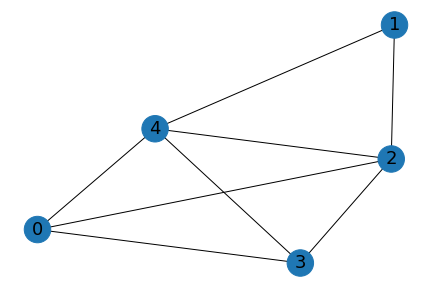
\includegraphics[width=0.5\linewidth]{imgs/greedyexx1.png} &   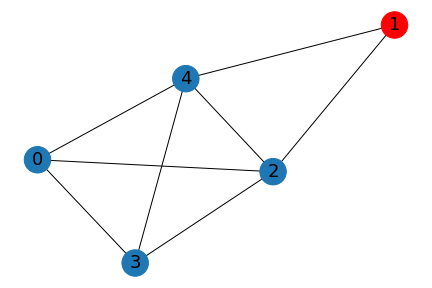
\includegraphics[width=0.5\linewidth]{imgs/greedyexx2.png} \\
			\end{tabular}
			\caption{Correct Greedy Estimate}
			\label{figure:greedysearchcorrect1}
		\end{figure}
			
		\begin{figure}[h]
			\begin{tabular}{cc}
				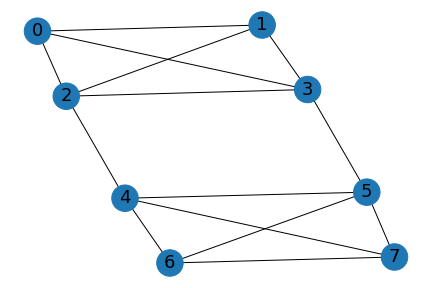
\includegraphics[width=0.5\linewidth]{imgs/greedycont1.png} &   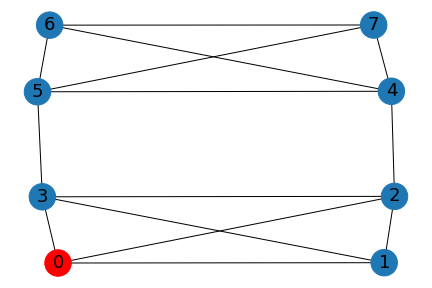
\includegraphics[width=0.5\linewidth]{imgs/greedycont2.png} \\
			\end{tabular}
			\caption{Wrong Greedy Estimate}
			\label{figure:greedysearchwrong1}
		\end{figure}
		
		The greedy algorithm will run more quickly than the exhaustive one. But the greedy algorithm does not guarantee an optimal solution to the problem. As analyzed above.
		
		\subsection{Compute Vertex Degree $Deg(u)$}
			\begin{algorithm}
				\caption{Compute Degree Of Vertex}
				\label{algorithm:GetVertexDegree}
				\SetKwInput{Input}{Input}                % Set the Input
				\SetKwInput{KwOutput}{Output}              % set the Output
				\DontPrintSemicolon
				
	%			\KwInput{$Adj(\mathcal{G})$}
				\Input{$Adj(\mathcal{G})$ \tcp*{adjacency matrix of $\mathcal{G}$}\\
					$vertex$ \tcp*{$vertex \in \mathcal{V}$}\\
				}
				
				\KwOutput{$degree$ \tcp*{degree of vertex $\in \mathcal{G}$}}
				
				% Set Function Names
				\SetKwFunction{FMain}{GetVertexDegree}
				
				% Function Definition			
				\SetKwProg{Fn}{Function}{:}{\KwRet}
				\Fn{\FMain}{%
					Set $degree \gets 0$ \;%
					\tcp{fetch row of vertex}
					\ForEach{$v_2 \in Adj(\mathcal{G})[vertex]$}{%
						\tcp{if edge exists}%
						\uIf{$v_2 == 1$}{%
							$degree = degree + 1$\;
						}					
					}
					\KwRet $degree$\;
				}
			\end{algorithm}
				
			This method computes the degree of a given vertex via the adjacency matrix. In this case, for a given vertex, we search through the remaining $(n-1)$ vertices which are on the columns of the adjacency matrix and where we have a one (1) value, then we have a neighbor of the vertex. So we count all the immediate neighbors of the given vertex and return the result. Clearly, since we do not have self loops for vertices in any arbitrary graph for this project, we search for neighboring vertices among the remaining $(n-1)$ vertices. Thus, our above algorithm runs in complexity $\mathbf{\mathcal{O}(n-1)}=\mathbf{\mathcal{O}(n)}$. 
		
		\subsection{Main Greedy Heuristic Method}
			\begin{algorithm}
				\caption{Greedy Heuristics}
				\label{algorithm:GreedyHeuristics}
				\SetKwInput{KwInput}{Input}                % Set the Input
				\SetKwInput{KwOutput}{Output}              % set the Output
				\DontPrintSemicolon
				
				\KwInput{$\mathcal{G(V,E)}$ \tcp*{Graph vertices $V$ edges $E$}}
				\KwOutput{$min\_cut$ \tcp*{minimum cut of $\mathcal{G}$}}
				
				% Set Function Names
				\SetKwFunction{FMain}{GreedyHeuristics}
				
				% Function Definition			
				\SetKwProg{Fn}{Function}{:}{\KwRet}
				\Fn{\FMain}{
					Set $min\_cut\_size \gets \infty$ \;%
					Set $min\_cut\_set \gets None$ \;
					\ForEach{$vertex \in \mathcal{V}$}{%
						$cut\_size \gets$ GetVertexDegree($vertex, \mathcal{A}(G)$) \; 
						\uIf{$cut\_size < min\_cut$}{
							$min\_cut\_size = cut\_size$\;
							$min\_cut\_set = (vertex, \mathcal{V}\backslash vertex),$
						}					
					}
					\KwRet $min\_cut\_set, min\_cut\_size$\;
				}
			\end{algorithm}
			
			This GreedyHeuristics method implements a search for the minimum cut which may be the actual value or not. For each vertex in the vertices set, a cut is computed as the number of immediate neighbors of the vertex (degree of vertex) in question. If the computed degree is smaller than the $min\_cut\_size$ value, then $min\_cut\_size$  value is replaced with the computed degree. The $min\_cut\_size$ value which represents the vertex with the minimum degree is returned hoping it is the actual minimum cut. \\
			
			There are $n$ vertices in the vertices set $\mathcal{V}$ and for each vertex, the \textbf{GetVertexDegree} method is called to compute the degree for the vertex in question which runs in $\mathbf{\mathcal{O}(n)}$, the complexity for this GreedyHeuristic technique implemented becomes
			\begin{align*}
				C =& \mathcal{O}(n\cdot n) \\
				C =& \mathbf{\mathcal{O}(n^2)}
			\end{align*}
	
	
	\section{Probabilistic And Randomized Implementation}
		In this module, unlike the ExhaustiveSearch technique which returns the exact minimum cut by considering all possible cuts of the graph, a random complementary partition is selected in a uniform fashion out of the $(2^n-2)$ different partitions. Since we know half of these partitions set are permutations, then the probability of realizing the exact minimum cut is at least 
		\begin{align*}
			\mathcal{P}=&\left(\dfrac{2}{2^n-2}\right) \\
			=&\dfrac{1}{2^{n-1}-1}
		\end{align*}
		 
		Reason simply being that, there exists a permutation of the actual minimum cut complementary partition.\\
		
		The implementation of this algorithm takes two (2) major steps. The idea is to randomly choose an edge from the graph and merge the vertices into a supernode, whilst updating the weight of the superedges connecting the newly formed supernode and neighbours of contributing vertices. This is repeated until a superedge remains in the graph connecting two (2) supernodes. The weight of this superedge represents the minimum cut of the graph.\\
		
		This algorithm utilizes two (2) functions
		\begin{itemize}
			\item Picking random edges to merge. $Algorithm\text{ }(\ref{algorithm:UpdateGraph}$)
			\item Updating the Graph. $Algorithm \text{ }(\ref{algorithm:probabilisticRandomized})$
		\end{itemize}
	
		
		\subsection{Merging Operation}
			\begin{algorithm}
				\caption{Merge Edge Update Graph}
				\label{algorithm:UpdateGraph}
				\SetKwInput{KwInput}{Input}                % Set the Input
				\SetKwInput{KwOutput}{Output}              % set the Output
				\DontPrintSemicolon
				
				\KwInput{$\mathcal{G(V,E)}$ \tcp*{graph to update}\\
					$(u, v)$ \tcp*{edge to merge $\in \mathcal{E}$}\\
				}
				\KwOutput{$\mathcal{G(V,E)}$ \tcp*{updated graph $\mathcal{G(V,E)}$}}
				
				% Set Function Names
				\SetKwFunction{FMain}{UpdateGraph}
				
				% Function Definition			
				\SetKwProg{Fn}{Function}{:}{\KwRet}
				\Fn{\FMain}{
					Set $supernode \gets $ string(`$u\cdot v$') \;%
					Set $updated\_graph \gets $ empty\_graph \;\;
	
					\tcp{fetch the neighbors of $u$ and $v$}
					u\_neighbors = $\mathcal{E}\cdot neighbors(u)$\;
					v\_neighbors = $\mathcal{E}\cdot neighbors(v)$\;\;
					
					\tcp{create superedge for $u$ edges}				
					\ForEach{$nb \in $ u\_neighbors}{%
						\uIf{$nb <> v$}{%
							edge\_weight = $w(\{u, nb \}\in \mathcal{E})$\;
							$\mathcal{E}\cdot $ add($nb, supernode, edge\_weight)$
						}							
					}\;
					\tcp{create superedge for $v$ edges}	
					\ForEach{$nb \in $ v\_neighbors}{%
						\uIf{$nb <> u$}{%
							\tcp{edge\_weight wt}
							wt = $w(\{v, neighbor\}\in \mathcal{E})$\;
							
							\tcp{update superedge's weight}
							\uIf{$(nb, supernode) \in \mathcal{E}$}{%
								$\mathcal{E}(nb, supernode).wt += wt$\;
							}\Else{
								$\mathcal{E}\cdot $add($nb, supernode, edge\_weight)$
							}
						}							
					}\;
					\tcp{edges updated, remove initial nodes}
					$\mathcal{E}\cdot remove\_edge(u,v)$ \;
					\KwRet $\mathcal{G(V,E)}$\;
				}
			\end{algorithm}
	
			From Algorithm (\ref{algorithm:UpdateGraph}), we realize that the edge contracting/merging is done on one (1) edge at a time, until only one edge remains in the graph. In the worst case, the neighbors of a vertex set could be $(n-1)$ which runs in $\mathcal{O}(n-1)=\mathbf{\mathcal{O}(n)}$.
		
		
		\subsection{Main Probability Randomized Method}
			\begin{algorithm}[h]
				\caption{Randomized Algorithm}
				\label{algorithm:probabilisticRandomized}
				\SetKwInput{KwInput}{Input}                % Set the Input
				\SetKwInput{KwOutput}{Output}              % set the Output
				\DontPrintSemicolon
				
				\KwInput{$\mathcal{G(V,E)}$ \tcp*{Graph vertices $\mathcal{V}$ edges $\mathcal{E}$}}
				\KwOutput{$min\_cut\_size$ \tcp*{minimum cut size of $\mathcal{G}$}\\
					$min\_cut\_set$\tcp*{minimum cut edges}
				}
				
				\SetKwRepeat{Do}{do}{while}
				
				% Set Function Names
				\SetKwFunction{FMain}{ProbabilisticRandomized}
				
				% Function Definition			
				\SetKwProg{Fn}{Function}{:}{\KwRet}
				\Fn{\FMain}{
					\While{$|\mathcal{E}| > 1$}{
						\tcp{choose random edge to merge}
						edge\_to\_merge = uniform$\cdot $random($\{e ; e \in \mathcal{E}\}$)\;
						$\mathcal{G(V,E,W)} = $ UpdateGraph($edge\_to\_merge, \mathcal{G(V,E,W)}$)
					}
					$min\_cut\_set = (u,v) \in \mathcal{E}$ \;
					$min\_cut\_size = \{w({u,v}) \in \mathcal{W}$\}\;
					\KwRet $min\_cut\_set, min\_cut\_size$\;
				}
			\end{algorithm}
			
			The \textbf{ProbabilityRandomized} in Algorithm (\ref{algorithm:probabilisticRandomized}) is the actual implementation of a randomized algorithm for the minimum cut. The algorithm merges vertices of a random edge one (1) at a time until only two (2) vertices are remaining. This runs in complexity $\mathcal{O}(n-2)=\mathcal{O}(n)$. The \textbf{UpdateGraph} method in Algorithm \ref{algorithm:UpdateGraph} runs at most for $(n-1)$ vertices. Thus, $\mathcal{O}(n)$ time. Putting all together, this algorithm runs in $\mathcal{O}(n\cdot n)=\mathbf{\mathcal{O}(n^2)}$\\
			
			On multiple runs of this algorithm, the minimum cut returned may be different from the previous estimate.\\
		
			\begin{figure}[h]
				\begin{tabular}{cc}
					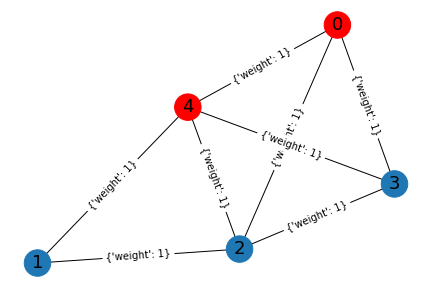
\includegraphics[width=0.5\linewidth]{imgs/probrandexx1.png} &   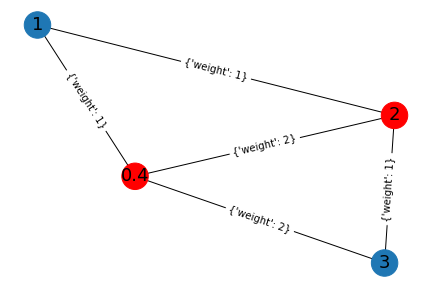
\includegraphics[width=0.5\linewidth]{imgs/probrandexx2.png} \\
					(a) 5 Nodes 8 Edges & (b) 4 Nodes 5 Edges \\[6pt]
					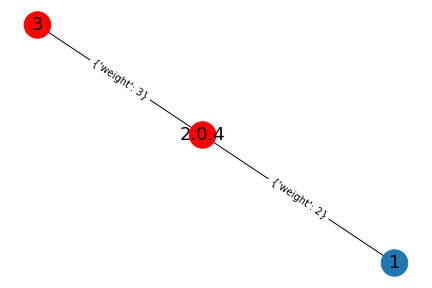
\includegraphics[width=0.5\linewidth]{imgs/probrandexx3.png} &   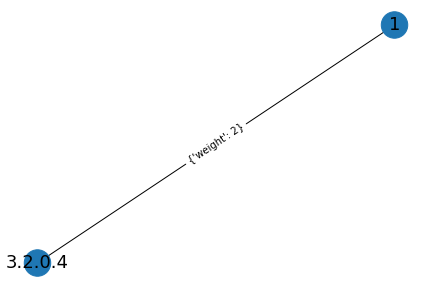
\includegraphics[width=0.5\linewidth]{imgs/probrandexx4.png} \\
					(c) 3 Nodes 3 Edges & (d) 2 Nodes 1 Edge \\[6pt]
				\end{tabular}
				\caption{Random Edge Contraction}
				\label{figure:randomedgecontractionexample1}
			\end{figure}
			
			
			Fig (\ref{figure:randomedgecontractionexample1}) is an implementation of the randomized algorithm as described in \textbf{ProbabilityRandomized} in Algorithm (\ref{algorithm:probabilisticRandomized}) above on a connected graph with five (5) vertices and eight (8) edges. The default weight of all edges in the graph is one (1). In each instance of the execution, an edge is picked at random and merged into a supernode, until only one edge is left. From the start to the finish of the algorithm, it is worth noting that, $(5-2)=3$ vertices were merged on. Also, the example happens to give the correct minimum cut, but only because we carefully picked the edges for merging. There are many other choices of edges for merging, so it's possible we could have ended with a cut with more than two (2) edges.\\
		
		\subsection{Improving Randomized Results}
			From the literature \cite{mincutandkargersalgorithm}, running the \textbf{ProbabilityRandomized} algorithm multiple times and returning the minimum cut results in a much higher probability of realizing the exact minimum cut. It was proved that, the number of trials to perform can be expressed as $\left(\mathcal{C}\cdot {n\choose 2}\cdot \ln (n)\right)$ so as to have a higher chance of realizing the minimum cut with probability of at least $$\mathcal{P}\ge 1-\dfrac{1}{n^C}$$
			The improved method is presented in Algorithm (\ref{algorithm:ImprovedProbabilisticRandomized}), with complexity, 
			\begin{align*}
				C &=\mathcal{O}\left(\mathcal{C}\cdot {n\choose 2}\cdot \ln (n) \cdot n^2 \right)\\
				&= \mathcal{O}\left(\dfrac{n(n-1)}{2}\cdot n^2\cdot \ln(n)\right)\\
				&=\mathcal{O}\left(n^4\cdot \ln(n)\right)
			\end{align*}
			
			\begin{algorithm}[h]
				\caption{Improved Randomized Algorithm}
				\label{algorithm:ImprovedProbabilisticRandomized}
				\SetKwInput{KwInput}{Input}                % Set the Input
				\SetKwInput{KwOutput}{Output}              % set the Output
				\DontPrintSemicolon
				
				\KwInput{$\mathcal{G(V,E)}$ \tcp*{Graph vertices $\mathcal{V}$ edges $\mathcal{E}$}}
				\KwOutput{$min\_cut\_size$ \tcp*{minimum cut size of $\mathcal{G}$}\\
					$min\_cut\_set$\tcp*{minimum cut edges}
				}
				
				\SetKwRepeat{Do}{do}{while}
				
				% Set Function Names
				\SetKwFunction{FMain}{ImpProbabilisticRandomized}
				
				% Function Definition			
				\SetKwProg{Fn}{Function}{:}{\KwRet}
				\Fn{\FMain}{
					$min\_cut\_size = \infty$\;
					$min\_cut\_set = None$\;
					Num\_Trials $= \mathcal{C}\cdot {n\choose 2}\cdot \ln (n)$\tcp*{$C \in \mathcal{N}, n=|\mathcal{V}|$}
					\ForEach{$trial \in $ Num\_Trials}{%
						cut\_set, cut\_size = ProbabilisticRandomized($\mathcal{G(V,E,W)}$)\;						
						\uIf{$min\_cut\_size < $ cut\_size}{%
							$min\_cut\_size = $ cut\_size\;
							$min\_cut\_set = $ cut\_set\;
						}							
					}
					\KwRet $min\_cut\_set, min\_cut\_size$\;
				}
			\end{algorithm}
		
		For simplicity sake, I chose the value of $\mathcal{C}=1$ which could be any positive integer.
		
	\section{Computational Complexities}
		For analysis purposes, only some graphs were selected for comparison of the various algorithms. 
		
		\subsection{Graphs Considered For Analysis}
			The graphs considered are presented in TABLE \ref{table:graphsconsidered}. From observation, any graph with vertices larger than twenty (20) takes infinitely long time to execute the Exhaustive-Search algorithm. The choice of the various graphs is done so as to realize some patterns among the executions of the various algorithms.
			
			\begin{table}[h]
				\caption{Graphs Considered}
				\label{table:graphsconsidered}
				{\renewcommand{\arraystretch}{2}
					\begin{center}
					\begin{tabular}{|c|c|c|}
						\hline
						Graph&Vertices&Edges \\
						\hline
						1&5&8\\
						\hline
						2&10&28\\
						\hline
						3&15&64\\
						\hline
						4&20&108\\
						\hline
						\textcolor{red}{5}&\textcolor{red}{25}&\textcolor{red}{168}\\
						\hline
					\end{tabular}
				\end{center}
				}
			\end{table}
		
		\subsection{Algorithms Complexities}
			It can be observed from Fig. (\ref{figure:complexities}) that, the complexity of the Exhaustive-Search algorithm for graphs having more than eighteen (18) vertices tend to increase very fast, as compared to the other algorithms. This explains why my computer (\textit{16GBRAM, AMD Ryzen 7 4800H with Radeon Graphics and speed 2.90 GHz}) had to restart automatically due to the expensive computational resource used up by the Exhaustive-Search algorithm when computing the minimum cut for graph with twenty-five (25) vertices. The Improved Probability Randomized algorithm has a reasonable running time compared to the Exhaustive Search. Since the Greedy and Probabilistic Randomized algorithms run have the same complexities, we didn't observe any significant difference in their running times. 
			\begin{table}[h]
				\caption{Complexities}
				\label{table:computationalComplexities}
				{\renewcommand{\arraystretch}{2}
					\begin{tabular}{|c|c|c|c|}
						\hline
						Brute-Force & Greedy & ProbRand & ImpProbRand\\
						\hline
						$\mathcal{O}\left(2^{2n}\right)$&
						$\mathcal{O}(n^2)$&$\mathcal{O}(n^2)$&$\mathcal{O}\left(n^4\cdot \ln(n)\right)$\\
						\hline
					\end{tabular}
				}
			\end{table}
			\begin{figure}[h]
				\begin{tabular}{cc}
					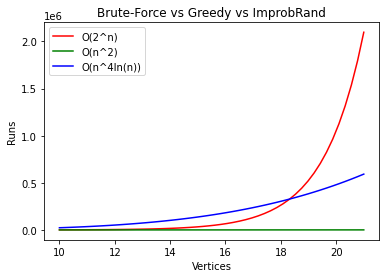
\includegraphics[width=0.5\linewidth]{imgs/complexitiesallalgs.png} &   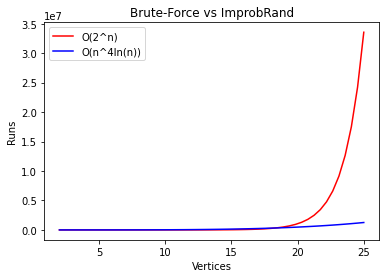
\includegraphics[width=0.5\linewidth]{imgs/complexitiesbruteforceimpprobrand.png} \\
				\end{tabular}
				
				\begin{center}
					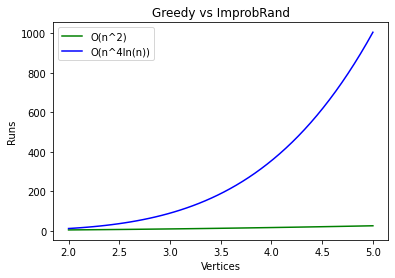
\includegraphics[width=0.5\linewidth]{imgs/complexitiesgreedyimpprobrand.png}
				\end{center}
				\caption{Graph Of Complexities}
				\label{figure:complexities}
			\end{figure}
		
		\subsection{Algorithms Timed Executions}
			The individual timing of execution for the algorithms is presented 
			
			\begin{itemize}
				\item Exhaustive Search
					\begin{table}[h]
						\caption{Timed Brute-Force}
						\label{table:timedbruteforce}
						\begin{center}					
						{\renewcommand{\arraystretch}{2}
							\begin{tabular}{|c|c|l|}
								\hline
								Graph& Time(sec) & Counter\\
								\hline
								1&0.002&112\\
								2&0.082&12544\\
								3&3.934&892928\\
								4&146.1&50855936\\
								\hline
							\end{tabular}
						}
						\end{center}
					\end{table}
					
					The number of iterations executed by the Brute-Force algorithm can formally be presented as 
					\begin{align*}
						C&=\sum_{i=1}^{2^n}1+\sum_{i=1}^{(2^{n-1}-1)}\cdot \sum\limits_{\substack{j=1 \\ S\subset \mathcal{V}}}^{|S|}\cdot 
						\sum\limits_{\substack{k=1 \\ T=\mathcal{V}\backslash S }}^{|T|} 1\\
						&=2^n+\left(2^{n-1}-1\right)\cdot |S|\cdot |T| \\
%						&\le 2^n+\left(2^{n-1}-1\right)\cdot \frac{n}{2}\cdot \frac{n}{2} \\
						&\le 2^n+\left(2^{n-1}-1\right)\cdot \frac{n^2}{4} \\
						&< 2^n+\left(2^{n-1}-1\right)\cdot n^2 \\
						&< 2^n+2^{n-1}\cdot n^2 \\
						&< 2^n+2^{n}\cdot n^2 \\
						&\le 2^{2n}\\
					\end{align*}
					As shown above, $C=2^{2n}$ is an upper bound to our minimum cut problem via the Brute-Force algorithm.
					
				\item Greedy-Heuristics
					\begin{table}[h]
						\caption{Timed Greedy-Heuristics}
						\label{table:timedgreedy}
						\begin{center}					
							{\renewcommand{\arraystretch}{2}
								\begin{tabular}{|c|c|l|}
									\hline
									Graph& Time(sec) & Counter\\
									\hline
									1&0.00099&25\\
									2&0.0&100\\
									3&0.001000&225\\
									4&0.001000&400\\
									5&0.000999&625\\
									\hline
								\end{tabular}
							}
						\end{center}
					\end{table}
					
					Again, the number of iterations executed by the Greedy-Heuristics algorithm can formally be presented as 
					\begin{align*}
						C&=\sum_{i=1}^{n}\cdot \sum_{j=1}^{n}1\\
						&=n\cdot n\\
						&=n^2
					\end{align*}
					As shown above, $C=n^2$ is the exact number of iterations for the Greedy-Heuristics in estimating the minimum cut size for a graph with $n$ vertices.
					
				\item Probabilistic Randomized Algorithm
					\begin{table}[h]
						\caption{Timed Greedy-Heuristics}
						\label{table:probrandom}
						\begin{center}					
							{\renewcommand{\arraystretch}{2}
								\begin{tabular}{|c|c|l|}
									\hline
									Graph& Time(sec) & Counter\\
									\hline
									1&0.0&16\\
									2&0.0&67\\
									3&0.0008&164\\
									4&0.002&281\\
									5&0.001&447\\
									\hline
								\end{tabular}
							}
						\end{center}
					\end{table}
					
					Every run of this algorithm results in $n-2$ merge operations. In each run, we check the $n$ vertices for connection to vertices to be merged for graph update. We construct an upper bound for this algorithm as follows 
					\begin{align*}
						C&=\sum_{i=1}^{(n-2)}\cdot \sum_{j=1}^{n} 1 \\
						&=(n-2)\cdot n\\
						&=n^2-2n \\
						&<n^2
					\end{align*}
					We hereby have an upper bound to our minimum cut problem with this random probabilistic implementation.
					
				\item Improved Probabilistic Randomized Algorithm \\
					\begin{table}[h]
						\caption{Timed Greedy-Heuristics}
						\label{table:impprobrandom}
						\begin{center}					
							{\renewcommand{\arraystretch}{2}
								\begin{tabular}{|c|c|l|}
									\hline
									Graph& Time(sec) & Counter\\
									\hline
									1&0.002&256\\
									2&0.035&6991\\
									3&0.199&45478\\
									4&0.652&158899\\
									5&1.685&422897\\
									\hline
								\end{tabular}
							}
						\end{center}
					\end{table}
					
					As implemented above for the Probabilistic Randomized algorithm \ref{table:probrandom}, an upper bound for this algorithm could be expressed as
					\begin{align*}
						C&< n\cdot C \cdot {n\choose 2} \ln (n)\\
					\end{align*}
			\end{itemize}
			
			
	\section{Auxiliary Functions}
		We employed four (4) functions to help with the implementation of this project. They are;
		\begin{enumerate}[label=\arabic*)]
			\item CreateDirectory
				\begin{itemize}
					\item create directories to hold graphs and plots.
					\item deletes directories as requested.
				\end{itemize}
			\item GenerateGraphs
				\begin{itemize}
					\item generates random Erdos Renyi graphs based on specified parameters. 
					\item plot graphs after generation
					\item save created graph to directory in current graphs directory.
				\end{itemize}
			\item LoadGraph
				\begin{itemize}
					\item load a graph from file.
					\item plot the graph if requested.
				\end{itemize}
			\item PlotGraph
				\begin{itemize}
					\item main implementation of graph plotting.
					\item weighted or not weighted.
					\item partly colored or not.
				\end{itemize}
		\end{enumerate}
		
		
	\bibliography{references} % use a field named url or \url{} for URLs
	% Note: the \bibliographystyle is set automatically
	
\end{document}
